\documentclass{beamer}
\usepackage{pythonhighlight}
\usepackage{syntax}
\newcommand{\BS}{\char`\\}
\grammarindent=0.28\textwidth
\usepackage{fourier}
\usepackage{tikz}
\usetikzlibrary{arrows,shapes,decorations,automata,backgrounds,positioning}
\usepackage{upgreek} % For \Pi
\usepackage{adjustbox}
%\usepackage{subfigure}
\usepackage{proof}
\usepackage{bbm}
\usepackage{listings}
\usepackage[colorinlistoftodos,prependcaption,textsize=tiny]{todonotes}\definecolor{LtGray}{rgb}{0.95,0.95,0.95}

\lstset{%
%language=Java,			% choose the language of the code
basicstyle=\scriptsize,	% the size of the fonts that are used for the code
columns=fullflexible,
mathescape=true,
tabsize=2, linewidth=\textwidth, 
numbers=left,				% where to put the line-numbers
numberstyle=\tiny,			% the size of the fonts that are used for the line-numbers
stepnumber=1,				% the step between two line-numbers. If it's 1 each line will be numbered
numbersep=5pt,			% how far the line-numbers are from the code
backgroundcolor=\color{LtGray},% choose the background color. You must add \usepackage{color}
showspaces=false,			% show spaces adding particular underscores
showstringspaces=false,		% underline spaces within strings
showtabs=false,			% show tabs within strings adding particular underscores
frame=lines,				% adds a frame around the code
tabsize=2,					% sets default tabsize to 2 spaces
captionpos=b,				% sets the caption-position to bottom
floatplacement={tbp},
breaklines=true,			% sets automatic line breaking
breakatwhitespace=false,		% sets if automatic breaks should only happen at whitespace
escapeinside={\%*}{*)},		% if you want to add a comment within your code
numberbychapter=false
}

\lstdefinestyle{padrao}{%
%language=Java,			% choose the language of the code
basicstyle=\scriptsize,	% the size of the fonts that are used for the code
columns=fullflexible,
mathescape=true,
tabsize=2, linewidth=\textwidth, 
numbers=left,				% where to put the line-numbers
numberstyle=\tiny,			% the size of the fonts that are used for the line-numbers
stepnumber=1,				% the step between two line-numbers. If it's 1 each line will be numbered
numbersep=5pt,			% how far the line-numbers are from the code
backgroundcolor=\color{LtGray},% choose the background color. You must add \usepackage{color}
showspaces=false,			% show spaces adding particular underscores
showstringspaces=false,		% underline spaces within strings
showtabs=false,			% show tabs within strings adding particular underscores
frame=lines,				% adds a frame around the code
tabsize=2,					% sets default tabsize to 2 spaces
captionpos=b,				% sets the caption-position to bottom
floatplacement={tbp},
breaklines=true,			% sets automatic line breaking
breakatwhitespace=false,		% sets if automatic breaks should only happen at whitespace
escapeinside={\%*}{*)},		% if you want to add a comment within your code
numberbychapter=false
}

\lstdefinestyle{maudedef}{%
%language=Java,			% choose the language of the code
basicstyle=\scriptsize\sffamily,	% the size of the fonts that are used for the code
columns=fullflexible,
mathescape=true,
tabsize=2, linewidth=\textwidth, 
showspaces=false,			% show spaces adding particular underscores
showstringspaces=false,		% underline spaces within strings
showtabs=false,			% show tabs within strings adding particular underscores
tabsize=2,					% sets default tabsize to 2 spaces
captionpos=b,				% sets the caption-position to bottom
floatplacement={tbp},
breaklines=true,			% sets automatic line breaking
breakatwhitespace=false,		% sets if automatic breaks should only happen at whitespace
escapeinside={\%*}{*)}		% if you want to add a comment within your code
}

\lstdefinelanguage{maude}{
 keywords={pr, ex, inc, fmod, endfm, mod, is, endm, sort, sorts, subsort, op, ops, eq, rl, ceq, if, then, else, fi, crl, assoc, comm, ctor, id, var, vars, mb, cmb}
}
\lstnewenvironment{maude}[1][]{\lstset{language=maude,style=padrao,#1}}{}
\lstnewenvironment{maudedef}[1][]{\lstset{language=maude,style=maudedef,#1}}{}

\lstdefinelanguage{piIR}{
 keywords={Blk, Bind, BindAbs, Id, Ref, Loop, Num, Ref, Abs, Call, Not, Eq, Assign, Mul, Sub, CSeq}
}
\lstnewenvironment{piIR}[1][]{\lstset{language=piIR,style=padrao,#1}}{}

\lstdefinelanguage{imp}{
 keywords={let, in, var, fn, while, not, do}
}
\lstnewenvironment{imp}[1][]{\lstset{language=imp,style=padrao,#1}}{}

\DeclareOptionBeamer{compress}{\beamer@compresstrue}
\ProcessOptionsBeamer

\mode<presentation>

\useoutertheme{infolines}
\useinnertheme{circles}
\usecolortheme{whale}
\usecolortheme{orchid}

\definecolor{blendedgreen}{rgb}{0,0.741,0.466}
\definecolor{green}{rgb}{0,0.4,0}

\setbeamercolor{structure}{fg=blendedgreen}
\setbeamercolor{titlelike}{parent=structure}
\setbeamercolor{frametitle}{fg=black}
\setbeamercolor{title}{fg=black}
\setbeamercolor{item}{fg=black}
\setbeamertemplate{caption}{\raggedright\insertcaption\par}

% Suppresses the ball and keeps the numbers in toc.
\setbeamertemplate{section in toc}{\inserttocsectionnumber.~\inserttocsection}

% Remove navigation buttons.
\beamertemplatenavigationsymbolsempty

\mode<all>

\logo{
\includegraphics[width=0.1\textwidth]{LogoIC-final.jpg}}

\usepackage{url}

\title[Compiler Construction with $\Pi$]{Notes on Formal Compiler Construction with the \\ \color{red}{$\Pi$ Framework}}
\author[C. Braga]{Christiano Braga} 
\institute[IC/UFF]{Instituto de Computa\c{c}\~ao, \\ Universidade Federal Fluminense, Niter\'oi, Brazil \\
}

\date{\today} 
\begin{document}

% ---

\begin{frame}[plain]

\titlepage

\begin{center}
\color{red}{\url{http://github.com/ChristianoBraga/PiFramework}}
\end{center}

\[
\includegraphics[width=0.2\textwidth]{LogoIC-final.jpg}\]

\end{frame}

% ---

\begin{frame}[plain]

\tiny
\tableofcontents

\end{frame}


% ---

%%%%%%%%%%%
\section{Introduction}
%%%%%%%%%%%

\begin{frame}{Compiler pipeline}

%\begin{adjustbox}{width=\textwidth,center}
%$\begin{array}{ccccccccccccc}
%source  & \xrightarrow{lexer} & tokens & \xrightarrow{parser} & concrete & \xrightarrow{AST \ transformer} & abstract & \xrightarrow{type \ checker} & abstract & \xrightarrow{code \ generator} & machine & \xrightarrow{optimizer} & optimized \\
%code    &            &        &             & syntax   &                      & syntax   &                   & syntax   &                     & code    & & machine \\
%        &            &        &             & tree     &                      & tree     &                   & tree     &                     &         & & code
%\end{array}$
%\end{adjustbox}

$$
\begin{array}{lllll}
p_L \xrightarrow{\mathit{lexical \ analysis}} \mathit{tokens}_p \\
\quad \qquad \qquad \xrightarrow{\mathit{syntactical \ analysis}} ast_p \\
\quad \qquad \qquad \qquad\qquad\xrightarrow{\mathit{semantic \ analysis}} ast_p \checkmark \\
\quad \qquad \quad \qquad \qquad \qquad\qquad\qquad\xrightarrow{\mathit{code \ generation}} p_{asm} \\
\quad \qquad \qquad \qquad \qquad \qquad \qquad\qquad\qquad\qquad\xrightarrow{\mathit{code \ optimization}} p'_{asm}
\end{array}
$$

\end{frame}

% --- 

\begin{frame}{Compiler pipeline and formal languages}

%\begin{adjustbox}{width=\textwidth,center}
%$\begin{array}{ccccccccccccc}
%        & Regular         &        & Context Free &          & Context Free         &          & Context Sensitive &          & Turing              &         & Turing & \\
%	& Grammar         &        & Grammar       &          & Grammar              &          & Grammar           &          & Machine             &         & Machine & \\
%source  & \xrightarrow{lexer} & tokens & \xrightarrow{parser}  & concrete & \xrightarrow{AST \ transformer} & abstract & \xrightarrow{type \ checker} & abstract & \xrightarrow{code \ generator} & machine & \xrightarrow{optimizer} & optimized \\
%code    &                 &        &              & syntax   &                      & syntax   &                   & syntax   &                     & code    & & machine \\
%        &                 &        &              & tree     &                      & tree     &                   & tree     &                     &         & & code
%\end{array}$
%\end{adjustbox}
$$
\begin{array}{lllll}
%
% Lexer
%
p_L
\xrightarrow{
  \scriptsize
  \begin{tabular}{c}
    \textit{lexical analysis} \\
    {\color{cyan}\textit{Linear Grm.}}
  \end{tabular}
} \mathit{tokens}_p \\
%
% Parser
%
\quad \quad \qquad
\xrightarrow{
\scriptsize
\begin{tabular}{c}
\textit{syntactical analysis} \\
{\color{cyan}\textit{Context-free Grm.}}
\end{tabular}
} ast_p \\
%
% Type-checker
%
\qquad \qquad \qquad \qquad\qquad
\xrightarrow{
\scriptsize
\begin{tabular}{c}
\textit{semantic analysis} \\
{\color{cyan}\textit{Context-sensitive Grm.}}
\end{tabular}
}
ast_p \checkmark \\
%
% Code generation
%
\quad \qquad \quad \qquad \qquad \qquad\qquad\qquad
\xrightarrow{
\scriptsize
\begin{tabular}{c}
\textit{code generation} \\
{\color{cyan}\textit{Context-sens. Grm.}}
\end{tabular}
}
p_{asm} \\
%
% Code optimization
%
\quad \qquad \qquad \qquad \qquad \qquad \qquad\qquad\qquad\qquad
\xrightarrow{
\scriptsize
\begin{tabular}{c}
\textit{code optimization} \\
{\color{cyan}\textit{Context-sens. Grm.}}
\end{tabular}
} p'_{asm}
\end{array}
$$


\end{frame}

% --- 

\begin{frame}[allowframebreaks]{Compiler pipeline with the {\color{red}$\Pi$ Framework}}

$$
p_L \xrightarrow{L_{\color{red} {\Pi_\mathit{Den}}}}
\begin{array}{c}
{p_{\color{red} {\Pi_\mathit{IR}}}} \\
\begin{adjustbox}{scale=1}
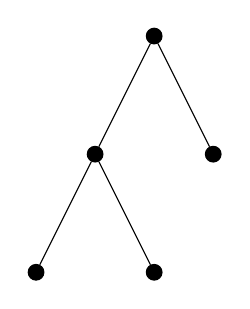
\begin{tikzpicture}
\tikzset{dot/.style={inner sep=2pt,circle,draw,fill}}
\node[dot](z){}
  child{node[dot]{}
    child{node[dot]{}}
    child{node[dot]{}}}
  child{node[dot]{}}
;
\end{tikzpicture}
\end{adjustbox}
\end{array}
\xrightarrow{{\color{red}\Pi_\delta}(p_{\color{red} {\Pi_\mathit{IR}}})}
\begin{array}{c}
{\llbracket p \rrbracket_{\color{red} {\Pi_\mathit{Aut}}}} \\
\begin{adjustbox}{scale=0.5}
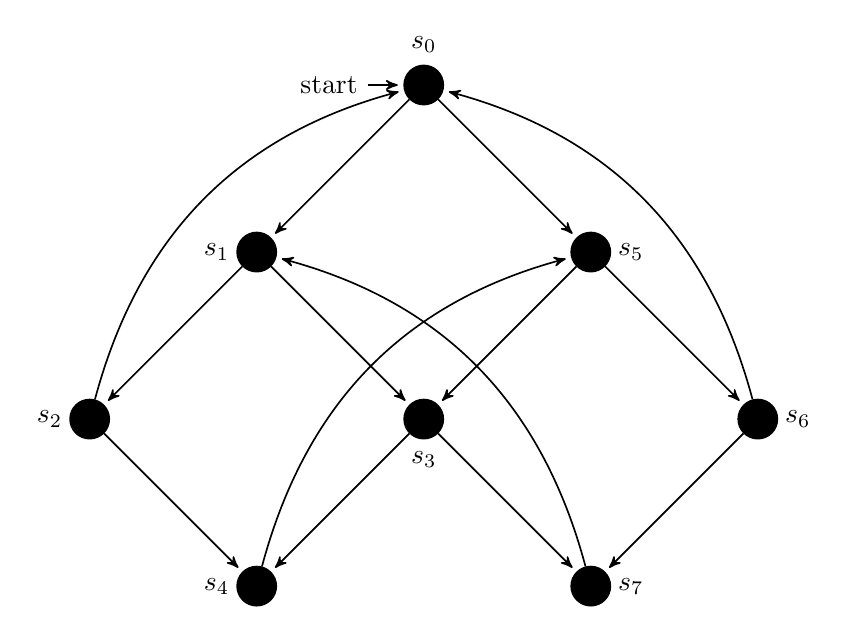
\begin{tikzpicture}
    [->,>=stealth',shorten >=2pt,auto,node distance=3cm, semithick,
     dot/.style={inner sep=5pt,circle,draw,fill}]
\node[initial, dot] (s0) {} ; \node at ([shift={(90:0.25)}] s0.90) {$s_0$};
\node[dot]           (s1) [below left of = s0] {}; \node at ([shift={(180:0.25)}] s1.180) {$s_1$};
\node[dot]           (s5) [below right of=s0] {}; \node at ([shift={(0:0.25)}] s5.0) {$s_5$};
\node[dot]           (s2) [below left of =s1] {}; \node at ([shift={(180:0.25)}] s2.180) {$s_2$};
\node[dot]           (s3) [below right of =s1] {}; \node at ([shift={(270:0.25)}] s3.270) {$s_3$};
\node[dot]           (s6) [below right of =s5] {}; \node at ([shift={(0:0.25)}] s6.0) {$s_6$};
\node[dot]           (s4) [below right of =s2] {}; \node at ([shift={(180:0.25)}] s4.180) {$s_4$};
\node[dot]           (s7) [below right of =s3] {}; \node at ([shift={(0:0.25)}] s7.0) {$s_7$};
\path (s0) edge (s1) edge (s5) ;
\path (s1) edge (s2) edge (s3) ;
\path (s5) edge (s3) edge (s6) ;
\path (s2) edge (s4) edge [bend left] (s0) ;
\path (s3) edge (s4) edge (s7) ;
\path (s4) edge [bend left] (s5) ;
\path (s6) edge [bend right] (s0) ;
\path (s6) edge (s7) ;
\path (s7) edge [bend right] (s1) ;
\end{tikzpicture}
\end{adjustbox}
\end{array}
$$

\newpage

\begin{adjustbox}{width=\textwidth,center}
$\begin{array}{ccccccccc}
             &                                                                                                                                                                                                                                                                                             &               &  \color{red}{\Pi} & \\
	     &                                                                                                                                                                                                                                                                                             &               &  \color{red}{Automata} & \\ \\
	     &                                                                           {\tiny Chomsky's \ hierarchy}                                                                                                                                                                                                                  &               &  \xrightarrow{interpreter} & output \\     
source  & {\tiny \xrightarrow{lexer} \circ \xrightarrow{parser}  \circ \xrightarrow{\stackrel{AST}{transformer}} \circ \xrightarrow{\stackrel{type}{checker}} \circ \xrightarrow{\stackrel{code}{generator}}} & \color{red}{\Pi \ IR} & \xrightarrow{code \ generator} & machine \ code \\
code             &                                                                                                                                                                                                                                                                                            &                 & \xrightarrow{model \ checker(P)} & counter\mbox{-}examples  \\
            &                                                                                                                                                                                                                                                                                             &                 & \text{\tiny where $P$ is a property}        &    \\
            &                                                                                                                                                                                                                                                                                             &                 & \text{\tiny in a suitable logic.}        &   \\           
\end{array}$
\end{adjustbox}

\begin{itemize}
\item {\color{red}$\Pi$ IR} defines a set of constructions common to many programming languages.
\item {\color{red}$\Pi$ IR} constructions have a formal automata-based semantics in {\color{red}$\Pi$ automata}.
\item One may execute (or validate) a program in a given language by running its associated {\color{red}$\Pi$ IR} program. 

\newpage

\item {\color{red}$\Pi$ Framework}: \url{http://github.com/ChristianoBraga/PiFramework}
\item Notes on Formal Compiler Construction with the {\color{red}$\Pi$ Framework}: \url{https://github.com/ChristianoBraga/PiFramework/blob/master/notes/notes.pdf}.
\end{itemize}


\end{frame}

%%%%%%%%%%%%
\subsection{Example}
%%%%%%%%%%%%

% ---
\begin{frame}[fragile]{A calculator}

We wish to compute simple arithmetic expressions such as $ 5 * (3 + 2)$.

\end{frame}

% ---

\begin{frame}[fragile]{A calculator: Lexer}
\begin{grammar}
<digit> ::= [0..9]

<digits> ::= <digit>$^+$

<boolean> ::= `true' | `false'
\end{grammar}
\end{frame}

% ---

\begin{frame}[fragile]{A calculator: concrete syntax}
\begin{grammar}
<exp> ::= <aexp> | <bexp>

<aexp> ::= <aexp> `+' <term> | <aexp> `-' <term> | <term>

<term> ::= <term> `*' <factor> | <term> `/' <factor> | <factor>

<factor> ::= `(' <aexp> `)'  | <digits>

<bexp> ::= <boolean> | `~' <bexp> | <bexp> <boolop> <bexp> 
\alt <aexp> <iop> <aexp>

<boolop> ::= `=' | `/\BS' | `\BS/'

<iop> ::= `<' | `>' | `<=' | `>=' 
\end{grammar}
\end{frame}

% ---

\begin{frame}[fragile]{A calculator: abstract syntax}
\begin{grammar}
<exp> ::= <digits> | <boolean> | <exp> <bop> <exp> 

<bop> ::= `+' | `-' | `*' | `/' | `=' | `\BS/`| `/\BS' | `<' | `>' | `<=' | `>=' 
\end{grammar}
\end{frame}

% ---

\begin{frame}[fragile, allowframebreaks]{A calculator: {\color{red}$\Pi$} denotations}
Let $D$ in <digits>, $B$ in <boolean> and $E_1, E_2$ in <exp>,

\begin{footnotesize}
\begin{align}
\label{eq:dig}\llbracket D \rrbracket_{\Pi} & = Num(D) \\
\llbracket B \rrbracket_{\Pi} & = Boo(B) \\
\label{eq:add}\llbracket E_1 + E_2 \rrbracket_{\Pi} & = Sum(\llbracket E_1 \rrbracket_{\Pi}, \llbracket E_2 \rrbracket_{\Pi}) \\
\llbracket E_1 - E_2 \rrbracket_{\Pi} & = Sub(\llbracket E_1 \rrbracket_{\Pi}, \llbracket E_2 \rrbracket_{\Pi}) \\
\label{eq:mul}\llbracket E_1 * E_2 \rrbracket_{\Pi} & = Mul(\llbracket E_1 \rrbracket_{\Pi}, \llbracket E_2 \rrbracket_{\Pi}) \\
\llbracket E_1 / E_2 \rrbracket_{\Pi} & = Div(\llbracket E_1 \rrbracket_{\Pi}, \llbracket E_2 \rrbracket_{\Pi}) \\
\llbracket E_1 < E_2 \rrbracket_{\Pi} & = Lt(\llbracket E_1 \rrbracket_{\Pi}, \llbracket E_2 \rrbracket_{\Pi}) \\
\llbracket E_1 {<=} E_2 \rrbracket_{\Pi} & = Le(\llbracket E_1 \rrbracket_{\Pi}, \llbracket E_2 \rrbracket_{\Pi}) \\
\llbracket E_1 > E_2 \rrbracket_{\Pi} & = Gt(\llbracket E_1 \rrbracket_{\Pi}, \llbracket E_2 \rrbracket_{\Pi}) \\
\llbracket E_1 {>\!=} E_2 \rrbracket_{\Pi} & = Ge(\llbracket E_1 \rrbracket_{\Pi}, \llbracket E_2 \rrbracket_{\Pi}) 
\end{align}
\end{footnotesize}

\framebreak 

\begin{itemize}
\item {\color{red}$\Pi$} denotations are \emph{functions} $\llbracket \cdot \rrbracket_\Pi : \mathit{AST} \to \Pi \ \mathit{IR}$, where 
\emph{AST} denotes the \emph{datatype} for the abstract syntax tree and $\Pi \ \mathit{IR}$ denotes the datatype for {\color{red}$\Pi \ \mathit{IR}$} programs. 
\item Note that $\llbracket \cdot \rrbracket_\Pi$ has \emph{trees} as parameters, instances of \emph{AST}. The example expression $5 * (3 + 2)$ becomes

\begin{adjustbox}{width=0.7\textwidth,center}
\begin{tikzpicture}[node distance=2.5cm,>=stealth', on grid]
\node (exp1) {$e_1$ : <exp>};
\node (exp2) [below left of = exp1] {$e_2$ : <exp>} ; 
\node (d1) [below of = exp2] {$5$ : <digits>} ; 
\node (op1) [right of = exp2] {* : <bop>} ;  
\node (exp3) [right of = op1] {$e_3$ : <exp>} ; 
\node (exp4) [right of = d1] {$e_4$ : <exp>} ; 
\node (d2) [below of = exp4] {$3$ : <digits>} ; 
\node (op2) [right of = exp4] {+ : <bop>} ;  
\node (exp5) [right of = op2] {$e_5$ : <exp>} ; 
\node (d3) [below of = exp5] {$2$ : <digits>} ; 

\path (exp1) edge node {} (exp2) edge node {} (op1) edge node {} (exp3) ;
\path (exp2) edge node {} (d1) ;
\path (exp3) edge node {} (exp4) edge node {} (op2) edge node {} (exp5) ;
\path (exp4) edge node {} (d2) ;
\path (exp5) edge node {} (d3) ; 
\end{tikzpicture}
\end{adjustbox}

\end{itemize}

\framebreak

\begin{footnotesize}
\begin{align*}
\llbracket 5 * (3 + 2) \rrbracket_{\Pi} & = Mul(\llbracket 5 \rrbracket_\Pi, \llbracket (3 + 2) \rrbracket_{\Pi}) & by \ Equation~\ref{eq:mul} \\
Mul(\llbracket 5 \rrbracket_\Pi, \llbracket (3 + 2) \rrbracket_{\Pi}) & = Mul(Num(5), \llbracket (3 + 2) \rrbracket_{\Pi}) & by \ Equation~\ref{eq:dig} \\
Mul(num(5), \llbracket (3 + 2) \rrbracket_{\Pi}) & = Mul(Num(5), Sum(\llbracket 3 \rrbracket_\Pi, \llbracket 2 \rrbracket_\Pi)  & by \ Equation~\ref{eq:add} \\
Mul(Num(5), Sum(\llbracket 3 \rrbracket_\Pi, \llbracket 2 \rrbracket_\Pi)  & =  Mul(Num(5), Sum(Num(3), \llbracket 2 \rrbracket_\Pi) & by \ Equation~\ref{eq:dig} \\
Mul(Num(5), Sum(Num(3), \llbracket 2 \rrbracket_\Pi)  & =  Mul(Num(5), Sum(Num(3), Num(2)) & by \ Equation~\ref{eq:dig} 
\end{align*}
\end{footnotesize}

\end{frame}

% --- 

\begin{frame}{A calculator: executing {\color{red}$\Pi$ IR} with {\color{red}$\Pi$ automata}}

A {\color{red}$\Pi$ automaton} is a $5$-tuple $\mathcal{A} = (G, Q, \delta, q_0, F)$, where $G$ is a context-free grammar, $Q$ is the set of states, $q_0$ is the initial state, $F \subseteq Q$ is the set of final states and
$$\delta : L(G)^* \times L(G)^* \times Store \to Q,$$ where $L(G)$ is the language generated by $G$ and $\mathit{Store}$ represents the memory. (Elements in a set $S^*$ are represented by terms $[s_1, s_2, \ldots, s_n]$.)

\begin{tiny}
\begin{align*}
\delta([Mul(Num(5), Sum(Num(3), Num(2)], \emptyset, \emptyset) & =  \delta([Num(5), Sum(Num(3), Num(2)), \#MUL], \emptyset, \emptyset) \\
\delta([Num(5), Sum(Num(3), Num(2)), \#MUL], \emptyset, \emptyset) & = \delta([Sum(Num(3), Num(2)), \#MUL], [Num(5)], \emptyset) \\ 
\delta([Sum(Num(3), Num(2)), \#MUL], [Num(5)], \emptyset) & = \delta([Num(3), Num(2), \#SUM, \#MUL], [Num(5)], \emptyset) \\
\delta([Num(3), Num(2), \#SUM, \#MUL], [Num(5)], \emptyset) & = \delta([Num(2), \#SUM, \#MUL], [Num(3), Num(5)], \emptyset) \\
\delta([Num(2), \#SUM, \#MUL], [Num(3), Num(5)], \emptyset) & = \delta([\#SUM, \#MUL], [Num(2), Num(3), Num(5)], \emptyset) \\
\delta([\#SUM, \#MUL], [Num(2), Num(3), Num(5)], \emptyset) & = \delta([\#MUL], [Num(5), Num(5)], \emptyset) \\
\delta([\#MUL], [Num(5), Num(5)], \emptyset) & = \delta(\emptyset, [Num(25)], \emptyset) \\
\delta(\emptyset, [Num(25)], \emptyset) & = Num(25)
\end{align*}
\end{tiny}
\end{frame}

%%%%%%%%%%%%%%%%
\section{$\Pi$ IR expressions}
%%%%%%%%%%%%%%%%

\subsection{Grammar}

% ---

\begin{frame}{Excerpt of  {\color{red}$\Pi$ IR} expressions}

\begin{grammar}
<Statement>  ::=  <Exp> 

<Exp>        ::=  <ArithExp> | <BoolExp> <Exp> 

<ArithExp>  ::=  `Num'(<digits>) | `Sum'(<Exp> , <Exp> ) |  `Sub'(<Exp>, <Exp>) | `Mul'(<Exp>, <Exp>) 

<BoolExp>  ::=  `Eq'(<Exp>, <Exp>) | `Not'(<Exp>)
\end{grammar}

\end{frame}

\subsection{Automaton}

% ---

\begin{frame}[allowframebreaks]{{\color{red}$\Pi$ automaton} semantics for {\color{red}$\Pi$ IR} expressions}
\begin{itemize}
\item Recall that $\delta : L(G)^* \times L(G)^* \times Store \to Q$, and let $N, N_i \in \mathbbm{N}$, $C, V \in L(G)^*$, $S \in \mathit{Store}$,
\begin{scriptsize}
\begin{align}
\delta(Num(N) :: C, V, S) & = \delta(C, Num(N) :: V, S) \\
\delta(Sum(E_1, E_2) :: C, V, S) & = \delta(E_1 :: E_2 :: \#SUM :: C, V, S) \\
\delta(\#SUM :: C, Num(N_1) :: Num(N_2) :: V, S) & = \delta(C, (N_1 + N_2) :: V, S) \\
\ldots \nonumber \\
\delta(Not(E) :: C, V, S) & = \delta(E :: \#NOT :: C, V, S) \\
\delta(\#NOT :: C, Boo(true) :: V, S) & = \delta(C, Boo(false) :: V, S) \\
\delta(\#NOT :: C, Boo(false) :: V, S) & = \delta(C, Boo(true) :: V, S) 
\end{align}
\end{scriptsize}

\item Notation $h :: ls$ denotes the concatenation of element $h$ with the list $ls$. 

\item $C$ represents the \emph{control} stack. $V$ represents the \emph{value} stack. $S$ denotes the memory store.

\item $\delta(\emptyset, V, S)$ denotes an \emph{accepting state}.

\item On a particular implementation of the $\Pi$ Framework, as in Python, \texttt{<digits>}
denote built-in numbers in implementation language, such that all arithmetic operations, such as \texttt{+}, are defined. 
That's why $N_i$ are in $\mathbbm{N}$.
\end{itemize}
\end{frame}

%%%%%%%%%%%%%%%
\section{$\Pi$ commands}
%%%%%%%%%%%%%%%

\subsection{Grammar}

% ---

\begin{frame}{{\color{red} $\Pi$ IR} commands}

\begin{itemize}
\item Commands are language constructions that require a \emph{memory} store to be evaluated. 
\begin{grammar}
<Statement> ::=  <Cmd> 

<Exp> := `Id`(<String>)

<Cmd>       ::=  `Assign'(<Id>, <Exp>) \alt `Loop'(<BoolExp>, <Cmd>) \alt  `CSeq'(<Cmd>, <Cmd>)
\end{grammar}


%\item From a syntactic standpoint, they extend both statements and expressions, as an identifier is an expression.
\end{itemize}

\end{frame}

\subsection{Automaton}

% ---

\begin{frame}[allowframebreaks,fragile]{{\color{red}$\Pi$ automaton} semantics for {\color{red}$\Pi$ IR} commands}
\begin{itemize}
\item A location $l \in Loc$ denotes a memory cell.
\item Storable and Bindable sets denote the data that may be mapped to by identifiers and locations on the memory and environment respectively. 
\item $Store = Loc \mapsto Storable$, $Env = Id \mapsto Bindable$, $Loc \subseteq Storable$, $\mathbbm{N} \subseteq Loc, Bindable$.
\item Now the transition function is $\delta : L(G)^* \times L(G)^* \times Env \times Store \to Q$, and let $W \in String$,  $C, V \in L(G)^*$, $S \in \mathit{Store}$, $E \in Env$, $B \in \mathit{Bindable}$, $l \in Loc$, $T \in \mathit{Storable}$, $X \in <Exp>$, $M, M_1, M_2 \in <Cmd>$,and expression $S' = S/[l \mapsto N]$ means that $S'$ equals to $S$ in all indices but $I$ that is bound to $N$,
\begin{tiny}
\begin{align}
\delta(Id(W) :: C, V, E, S) & = \delta(C, B :: V, E, S), \\ & \text{\bf where}~ E[W] = l ~\text{and}~ S[l] = B,\nonumber \\
%
\delta(Assign(W, X) :: C, V, E, S) & =  \delta(X :: \#ASSIGN :: C, W :: V, E, S'), \\
\delta(\#ASSIGN :: C, T :: W :: V, E, S) & = \delta(C, V, E, S'), & \\ & \text{\bf where}~ E[W] = l ~\text{and}~ S' = S/[l \mapsto T], \nonumber \\
%
\delta(Loop(X, M) :: C, V, E, S) & =  \delta(X :: \#LOOP :: C, Loop(X, M) :: V, E, S),  \\
\delta(\#LOOP :: C, Boo(true) :: Loop(X, M) :: V, E, S) & = \delta(M :: Loop(X, M) :: C, V, E, S),  \\
\delta(\#LOOP :: C, Boo(false) :: Loop(X, M) :: V, E, S) & = \delta(C, V, E, S), \\
%
\delta(CSeq(M_1, M_2) :: C, V, E, S) & = \delta(M_1 :: M_2 :: C, V, E, S).
\end{align}
\end{tiny}
\end{itemize}
\end{frame}

%%%%%%%%%%%%%%%%%%%%%%%%%
\section{$\Pi$ IR declarations}
%%%%%%%%%%%%%%%%%%%%%%%%%

\subsection{Grammar}

% ---

\begin{frame}{{\color{red}$\Pi$ IR} declarations}

\begin{itemize}
\item Declarations are statements that create an environment, binding identifiers to (bindable) values.
\item In {\color{red}$\Pi$ IR}, a bindable value is either a Boolean value, an integer or a location.
\item From a syntactic standpoint, all classes are monotonically extended.
\begin{grammar}
<Statement> ::= <Dec> 

<Exp>       ::=  `Ref'(<Exp>)> | `DeRef'(<Id>) | `ValRef'(<Id>)

<Dec>       ::= `Bind'(<Id>, <Exp>) | `DSeq'(<Dec>, <Dec>)

<Cmd>      ::= `Blk'(<Dec>, <Cmd>) 
\end{grammar}
\end{itemize}

\end{frame}

\subsection{Automaton}

% ---

\begin{frame}[allowframebreaks,fragile]{{\color{red}$\Pi$ automaton} semantics for {\color{red}$\Pi$ IR} declarations}

Let $\mathit{BlockLocs} = \mathcal{P}(\mathit{Loc})$, now the transition function is $\delta : L(G)^* \times L(G)^* \times Env \times Store \times \mathit{BlockLocs} \to Q$, and let $L, L' \in \mathit{BlockLocs}$, $\mathit{Loc} \subseteq \mathit{Storable}$, and $S / L$ means the store $S$ without the locations in $L$,

\begin{tiny}
\begin{align}
% References
\delta(Ref(X) :: C, V, E, S, L) & = \delta(X :: \#REF :: C, V, E, S, L), \\
\delta(\#REF :: C, T :: V, E, S, L) & = \delta(C, l :: V, E, S', L'), \text{\bf where } S' = S \cup [l \mapsto T], l \not\in S, L' = L \cup \{l\}, \\ \nonumber \\
% Dereference
\delta(DeRef(Id(W)) :: C, V, E, S, L) & = \delta(C, l :: V, E, S, L), \text{\bf where } l = E[W],  \\ \nonumber \\
% Reference value
\delta(ValRef(Id(W)) :: C, V, E, S, L) & = \delta(C, T :: V, E, S, L), \text{\bf where } T = S[S[E[W]]],  \\ \nonumber \\
% Bind
\delta(Bind(Id(W), X) :: C, V, E, S, L) &= \delta(X :: \#BIND :: C, W :: V, E, S, L), \\
\delta(\#BIND :: C, B :: W :: E' :: V, E, S, L) &= \delta(C, ([W \mapsto B] \cup E') :: V, E, S, L), \text{\bf where } E' \in \mathit{Env},\\
\delta(\#BIND :: C, B :: W :: H :: V, E, S, L) &= \delta(C, [W \mapsto B] :: H :: V, E, S, L), \text{\bf where } H \not\in \mathit{Env},  \\ \nonumber \\
% DSeq
\delta(DSeq(D_1, D_2), X) :: C, V, E, S, L) &= \delta(D_1 :: D_2 :: C, V, E, S, L), \\ \nonumber \\
% Block
\delta(Blk(D, M) :: C, V, E, S, L) &= \delta(D :: \#BLKDEC :: M :: \#BLKCMD :: C, L :: V, E, S, \emptyset), \\
\delta(\#BLKDEC :: C, E' :: V, E, S, L) &= \delta(C, E :: V, E / E', S, L), \\
%\delta(\#DEC :: C, m :: V, E, S, L) &= \delta(C, E :: V, E / m, S, L), \text{ where } m \in (\mathit{Id} \mapsto \mathit{Bindable}),\\
\delta(\#BLKCMD :: C, E :: L :: V, E', S, L') &= \delta(C, V, E, S', L), \text{ \bf where } S' = S / L.
\end{align}
\end{tiny}

\end{frame}

%%%%%%%%%%%%%%%%%%%%%%%%%
\section{$\Pi$ IR abstractions}
%%%%%%%%%%%%%%%%%%%%%%%%%

\subsection{Grammar}

% ---

\begin{frame}{{\color{red}$\Pi$ IR} abstractions}

\begin{itemize}
\item Abstractions extend Bindables by allowing a name to be bound to a list of formal parameters, a list of identifiers, and a block in the environment.
\item Such names can be called and applied to actual parameters, a list of expressions.
\begin{grammar}
<Dec>       ::= `Bind'(<Id>, <Abs>) 

<Abs>       ::= `Abs'(<Formals>, <Blk>) 

<Formals> ::= <Id>$^*$

<Cmd> ::= `Call`(<Id>, <Actuals>)

<Actuals> ::= <Exp>$^*$
\end{grammar}
\end{itemize}

\end{frame}

\subsection{Automaton}

\begin{frame}[allowframebreaks,fragile]{{\color{red}$\Pi$ automaton} semantics for {\color{red}$\Pi$ IR} abstractions --- Closures}

We chose a \emph{static binding} semantics for abstractions. Therefore, we interpret abstractions as \emph{closures} formed by an abstraction together with its declaration environment which defines the context in which the abstraction will be evaluated.

\[
\mathit{Closure} : \mathit{Formals} \times \mathit{Blk} \times \mathit{Env} \to \mathit{Bindable}
\]

\end{frame}

% ---

\begin{frame}[allowframebreaks,fragile]{{\color{red}$\Pi$ automaton} semantics for {\color{red}$\Pi$ IR} abstractions --- Example}
\begin{imp}
Im$\Pi$ source code:
# In this example we encapsulate the iterative calculation
# of the factorial within a function call.
let var z = 1
in
    let fn f(x) =
        let var y = x
        in
            while not (y == 0)
            do
                z := z * y
                y := y - 1
    in f(10)
\end{imp}
    
 \framebreak   

\begin{piIR}
$\Pi$ IR AST: 
Blk(Bind(Id(z), Ref(Num(1))), 
	Blk(Bind(Id(f), Abs(Id(x), 
		Blk(Bind(Id(y), Ref(Id(x))), 
			Loop(Not(Eq(Id(y), Num(0))), 
				CSeq(Assign(Id(z), Mul(Id(z), Id(y))), 
						Assign(Id(y), Sub(Id(y), Num(1)))))))), 
		Call(Id(f), Num(10))))
\end{piIR}
\end{frame}

% ---

\begin{frame}[allowframebreaks,fragile]{{\color{red}$\Pi$ automaton} semantics for {\color{red}$\Pi$ IR} abstractions}


%Let $\mathit{BlockLocs} = \mathit{Set}\{\mathit{Loc}\}$, now the transition function is $\delta : L(G)^* \times L(G)^* \times Env \times Store \times \mathit{BlockLocs} \to Q$, and let $L, L' \in \mathit{BlockLocs}$, $\mathit{Loc} \subseteq \mathit{Storable}$, and $S / L$ means the store $S$ without the locations in $L$,

Let $F \in \mathit{Formals}$, $B \in Blk$, $I \in \mathit{Id}$, $A \in \mathit{Actuals}$, $V_i \in \mathit{Value}$, $1 \le i \le n$, $n \in \mathbbm{N}$,

\begin{small}
\begin{align}
\delta(\mathit{Abs}(F, B) :: C, V, E, S, L) = \delta(C, \mathit{Closure}(F, B, E) :: V, E, S, L) 
\end{align}

\begin{align}
\delta(\mathit{Call}(I, [X_1, X_2, \ldots, X_n])) :: C, V, E, S, L) & = \\ \nonumber 
\delta(X_n :: X_{n-1} :: \ldots :: X_1 :: \#\mathit{CALL}(I, n) :: C&, V, E, S, L) 
\end{align}

\begin{align}
\delta(\#\mathit{CALL}(I, n) ::C&, (V_1 :: V_2 :: \ldots V_n :: V), E, S, L) = \\ \nonumber
	\delta(B :: \#BLKCMD :: C&, E :: V, E', S, L) \\ \nonumber
\text{\bf where } E &= \{I \mapsto \mathit{Closure}(F, B, E_1)\} \cup E_2,  \\  \nonumber
E' & = E / E_1 / \mathit{match}(F,  [V_1, V_2, \ldots, V_n]) 
\end{align}

\begin{align*}	
\mathit{match} : \mathit{Id^*} \times \mathit{Values^*} & \to \mathit{Env} \\ 
\mathit{match}(fl, al) & = \mathbf{if} |fl| \not= |al| \ \mathbf{than} \ \{\} \ \mathbf{else} \ \_\mathit{match}(fl, al, \{\}) \\ \\
\_\mathit{match} : \mathit{Id^*} \times \mathit{Values^* } \times \mathit{Env} & \to \mathit{Env} \\ 
\_\mathit{match}([], [], E) & = E \\
\_\mathit{match}(f, a, E)  & = \{f \mapsto a\} \cup E \\
\_\mathit{match}(f :: fl, a :: al, E) & = \_\mathit{match}(fl, al, \{f \mapsto a\} \cup E) 
\end{align*}
\end{small}

\end{frame}

%%%%%%%%%%%%%%%%%%%%%%%%%
\section{$\Pi$ IR recursive abstractions}
%%%%%%%%%%%%%%%%%%%%%%%%%

\subsection{Grammar}

% ---

\begin{frame}{{\color{red}$\Pi$ IR} recursive abstractions}

\begin{itemize}

\item Abstractions can be recursive to allow for the declaration of recursive functions.

\begin{grammar}
<Dec>       ::= `Rbnd'(<Id>, <Abs>) 
\end{grammar}
\end{itemize}

\end{frame}

\subsection{Automaton}

% ----

\begin{frame}[allowframebreaks,fragile]{{\color{red}$\Pi$ automaton} semantics for {\color{red}$\Pi$ IR} recursive abstractions --- Recursive closures}

In the context of \emph{static binding} semantics for abstractions, in a call to a recursive function, the evaluation of identifiers needs to be reminded about the binding of the function name to a closure.  

\begin{align*}
\mathit{Rec} &: \mathit{Formals} \times \mathit{Blk} \times \mathit{Env}  \times \mathit{Env} \to \mathit{Bindable} \\
\mathit{unfold} &: \mathit{Env} \to \mathit{Env} \\
\mathit{reclose}_E &: \mathit{Env} \to \mathit{Env} 
\end{align*}

\begin{align}
unfold(E) &= reclose_E(E) \\ 
reclose_E(I \mapsto Closure(F, B, E')) &= (I \mapsto Rec(F, B, E', E)) \\ 
reclose_E(I \mapsto Rec(F, B, E',E'')) & = (I\mapsto Rec(F, B, E', E)) \\ 
reclose_E(I\mapsto v) & = (I\mapsto v) \text{ if } v \not= Closure(F, B, E) \\
reclose_E(E_1\cup E_2) & = reclose_E(E_1) \cup reclose_E(E_2) \\ 
reclose_E(\emptyset) & = \emptyset
\end{align}

\end{frame}

% ---

\begin{frame}[allowframebreaks,fragile]{{\color{red}$\Pi$ automaton} semantics for {\color{red}$\Pi$ IR} recursive abstractions --- Recursive closures}

\begin{small}
\begin{align}
\delta(\mathit{Rbnd}&(I, Abs(F, B)) :: C, V, E, S, L)  = \nonumber \\ & \delta(C, \mathit{unfold}(I \mapsto \mathit{Closure}(F, B, E)) :: V, E, S, L) \\
\delta(\#\mathit{CALL}(I, n) ::C & , V_1 :: V_2 :: \ldots :: V_n :: V, E, S, L) = \nonumber \\
	& \delta(B :: \#\mathit{BLKCMD} :: C, E :: V, E', S, L) \\
\text{\bf where } E & =  \{I \mapsto \mathit{Rec}(F, B, E_1, E_2)\} \cup E_3, \nonumber \\
E'  & = E / E_1 / unfold(E_2) / \mathit{match}(F,  [V_1, V_2, \ldots, V_n]) \nonumber
\end{align}
\end{small}

\end{frame}

%%%%%%%%%%%%%%%%%%%%%%%%%
\section{$\Pi^2$: $\Pi$ Framework in Python}
%%%%%%%%%%%%%%%%%%%%%%%%%

\subsection{Expressions}

% ---
\begin{frame}[allowframebreaks,fragile]{{\color{red}$\Pi$ IR} expressions in Python}

%{\footnotesize\url{https://nbviewer.jupyter.org/github/ChristianoBraga/PiFramework/blob/master/python/pi.ipynb}}

\begin{python}
class Statement: 
    def __init__(self, *args):
        self.opr = args
    def __str__(self):
        ret = str(self.__class__.__name__)+"("
        for o in self.opr:
            ret += str(o)
        ret += ")"
        return ret
class Exp(Statement): pass
class ArithExp(Exp): pass
\end{python}

\framebreak

\begin{python}
class Num(ArithExp): 
    def __init__(self, f): 
        assert(isinstance(f, int))
        ArithExp.__init__(self,f)
class Sum(ArithExp): 
    def __init__(self, e1, e2): 
        assert(isinstance(e1, Exp) and isinstance(e2, Exp))
        ArithExp.__init__(self, e1, e2)
$\ldots$
\end{python}

\framebreak

\begin{python}
class BoolExp(Exp): pass
class Eq(BoolExp):
    def __init__(self, e1, e2):
        assert(isinstance(e1, Exp) and isinstance(e2, Exp))
        BoolExp.__init__(self, e1, e2)
$\ldots$
\end{python}

\framebreak

\begin{python}
exp = Sum(Num(1), Mul(Num(2), Num(4)))
print(exp)

Sum(Num(1)Mul(Num(2)Num(4)))
\end{python}

\framebreak

\begin{python}
exp2 = Mul(2, 1)
---------------------------------------------------------------------------
AssertionError                            Traceback (most recent call last)
<ipython-input-7-00fd40a79a54> in <module>()
----> 1 exp2 = Mul(2, 1)

<ipython-input-5-42a82e58862f> in __init__(self, e1, e2)
     28 class Mul(ArithExp):
     29     def __init__(self, e1, e2):
---> 30         assert(isinstance(e1, Exp) and isinstance(e2, Exp))
     31         ArithExp.__init__(self, e1, e2)
     32 class BoolExp(Exp): pass

AssertionError: 
\end{python}
\end{frame}

% ---

\begin{frame}[allowframebreaks,fragile]{{\color{red}$\Pi$ automaton} for {\color{red}$\Pi$ IR} expressions}

\begin{python}
## Expressions
class ValueStack(list): pass
class ControlStack(list): pass
class ExpKW:
    SUM = "#SUM"
    SUB = "#SUB"
    MUL = "#MUL"
    EQ = "#EQ"
    NOT = "#NOT"
\end{python}

\framebreak    

\begin{python}    
class ExpPiAut(dict):
    def __init__(self):    
        self["val"] = ValueStack()
        self["cnt"] = ControlStack()
    def __evalSum(self, e):
        e1 = e.opr[0]
        e2 = e.opr[1]
        self.pushCnt(ExpKW.SUM)
        self.pushCnt(e1)
        self.pushCnt(e2)
    def pushCnt(self, e):
        cnt = self.cnt()
        cnt.append(e)
$\ldots$
\end{python}

\framebreak

\begin{python}    
ea = ExpPiAut()
print(exp)
ea.pushCnt(exp)
while not ea.emptyCnt():
    ea.eval()
    print(ea)
\end{python}

\framebreak

\begin{adjustbox}{width=2\textwidth}
\begin{python}    
Sum(Num(1)Mul(Num(2)Num(4)))
{'val': [], 'cnt': ['#SUM', <__main__.Num object at 0x111851470>, <__main__.Mul object at 0x1118516d8>]}
{'val': [], 'cnt': ['#SUM', <__main__.Num object at 0x111851470>, '#MUL', <__main__.Num object at 0x111851630>, <__main__.Num object at 0x1118516a0>]}
{'val': [4], 'cnt': ['#SUM', <__main__.Num object at 0x111851470>, '#MUL', <__main__.Num object at 0x111851630>]}
{'val': [4, 2], 'cnt': ['#SUM', <__main__.Num object at 0x111851470>, '#MUL']}
{'val': [8], 'cnt': ['#SUM', <__main__.Num object at 0x111851470>]}
{'val': [8, 1], 'cnt': ['#SUM']}
{'val': [9], 'cnt': []}
\end{python}
\end{adjustbox}

\end{frame}

\subsection{Commands}

% ---

\begin{frame}[allowframebreaks,fragile]{{\color{red}$\Pi$ IR} commands}

\begin{adjustbox}{width=0.8\textwidth}
\begin{python}
class Cmd(Statement): pass
class Id(Exp):
    def __init__(self, s):
        assert(isinstance(s, str))
        Exp.__init__(self, s)
class Assign(Cmd):
    def __init__(self, i, e): 
        assert(isinstance(i, Id) and isinstance(e, Exp))
        Cmd.__init__(self, i, e)
class Loop(Cmd):
    def __init__(self, be, c):
        assert(isinstance(be, BoolExp) and isinstance(c, Cmd))
        Cmd.__init__(self, be, c)
class CSeq(Cmd):
    def __init__(self, c1, c2):
        assert(isinstance(c1, Cmd) and isinstance(c2, Cmd))
        Cmd.__init__(self, c1, c2)
\end{python}
\end{adjustbox}

\framebreak
        
\begin{python}
cmd = Assign(Id("x"), Num(1))
print(type(cmd))
print(cmd)
<class '__main__.Assign'>
Assign(Id(x)Num(1))
\end{python}
\end{frame}

% ---

\begin{frame}[allowframebreaks,fragile]{{\color{red}$\Pi$ automaton} for {\color{red}$\Pi$ IR} commands}

Environment, Location, Store and commands opcodes.

\begin{python}
## Commands
class Env(dict): pass
class Loc(int): pass
class Sto(dict): pass
class CmdKW:
    ASSIGN = "#ASSIGN"
    LOOP = "#LOOP"
\end{python}

\framebreak

{\color{red}$\Pi$ automaton} for commands extends the {\color{red}$\Pi$ automaton}  for expressions.

\begin{python}    
class CmdPiAut(ExpPiAut): 
    def __init__(self):    
        self["env"] = Env()
        self["sto"] = Sto()
        ExpPiAut.__init__(self)
    def env(self):
        return self["env"]
    def getLoc(self, i):
        en = self.env()
        return en[i]
    def sto(self):
        return self["sto"]
    def updateStore(self, l, v):
        st = self.sto()
        st[l] = v
\end{python}

\framebreak
        
{\color{red}$\Pi$}  semantics for assignment.

\begin{scriptsize}
\begin{align}
\delta(Assign(W, X) :: C, V, E, S) & = \delta(X :: \#ASSIGN :: C, W :: V, E, S'), \nonumber \\
\delta(\#ASSIGN :: C, T :: W :: V, E, S) & = \delta(C, V, E, S'), & \nonumber \\ & \text{\bf where}~ E[W] = l ~\text{and}~ S' = S/[l \mapsto T]. \nonumber
\end{align}
\end{scriptsize}

\begin{python}
    def __evalAssign(self, c): 
        i = c.opr[0]
        e = c.opr[1]
        self.pushVal(i.opr[0])
        self.pushCnt(CmdKW.ASSIGN)
        self.pushCnt(e)
    def __evalAssignKW(self):
        v = self.popVal()
        i = self.popVal()
        l = self.getLoc(i)
        self.updateStore(l, v) 
\end{python}

\framebreak

{\color{red}$\Pi$}  semantics for identifiers.
        
\begin{scriptsize}
\begin{align}
\delta(Id(W) :: C, V, E, S) & = \delta(C, B :: V, E, S), \nonumber \\ & \text{\bf where}~ E[W] = l ~\text{and}~ S[l] = B. \nonumber 
\end{align}
\end{scriptsize}
        
\begin{python}
    def __evalId(self, i):
        s = self.sto()
        l = self.getLoc(i)
        self.pushVal(s[l])
\end{python}

\framebreak
       
{\color{red}$\Pi$}  semantics for loop: recursive step.

\begin{scriptsize}
\begin{align}
\delta(Loop(X, M) :: C, V, E, S) & = \delta(X :: \#LOOP :: C, Loop(X, M) :: V, E, S). \nonumber 
\end{align}
\end{scriptsize}
       
\begin{python}
    def __evalLoop(self, c):
        be = c.opr[0]
        bl = c.opr[1]
        self.pushVal(Loop(be, bl))
        self.pushVal(bl)
        self.pushCnt(CmdKW.LOOP)
        self.pushCnt(be)
\end{python}

\framebreak
       
{\color{red}$\Pi$}  semantics for loop: basic steps.

\begin{scriptsize}
\begin{align}
\delta(\#LOOP :: C, Boo(true) :: Loop(X, M) :: V, E, S) & = \delta(M :: Loop(X, M) :: C, V, E, S), \nonumber \\
\delta(\#LOOP :: C, Boo(false) :: Loop(X, M) :: V, E, S) & = \delta(C, V, E, S). \nonumber
\end{align}
\end{scriptsize}
       
\begin{python}
    def __evalLoopKW(self):
        t = self.popVal()
        if t:
            c = self.popVal()
            lo = self.popVal()
            self.pushCnt(lo)
            self.pushCnt(c)
        else:
            self.popVal()
            self.popVal()
\end{python}

\framebreak

{\color{red}$\Pi$}  semantics for command composition.

\begin{scriptsize}
\begin{align}
\delta(CSeq(M_1, M_2) :: C, V, E, S) & = \delta(M_1 :: M_2 :: C, V, E, S). \nonumber
\end{align}
\end{scriptsize}

\begin{python}
    def __evalCSeq(self, c):
        c1 = c.opr[0]
        c2 = c.opr[1]
        self.pushCnt(c2)
        self.pushCnt(c1)
\end{python}

\framebreak

Commands are now on the top of the food chain.

\begin{python}
    def eval(self): 
        c = self.popCnt()
        if isinstance(c, Assign):
            self.__evalAssign(c)
        elif c == CmdKW.ASSIGN:
            self.__evalAssignKW()
        elif isinstance(c, Id):
            self.__evalId(c.opr[0])
        elif isinstance(c, Loop):
            self.__evalLoop(c)
        elif c == CmdKW.LOOP:
            self.__evalLoopKW()
        elif isinstance(c, CSeq):
            self.__evalCSeq(c)
        else:
            self.pushCnt(c)
            ExpPiAut.eval(self)
\end{python}
\end{frame}

% ---

\subsection{Declarations}
\begin{frame}[allowframebreaks,fragile]{{\color{red}$\Pi$ IR} declarations in Python}

\flushright{\fbox{\texttt{DeRef} and \texttt{ValRef} not implemented yet.}}

\begin{python}
## Declarations
class Dec(Statement): pass
class Bind(Dec):
   def __init__(self, i, e):
       assert (isinstance(i, Id) and isinstance(e, Exp))
       Dec.__init__(self, i, e)
class Ref(Exp):
   def __init__(self, e):
       assert (isinstance(e, Exp))
       Exp.__init__(self, e)
class Blk(Cmd):
   def __init__(self, d, c):
       assert (isinstance(d, Dec) and isinstance(c, Cmd))
       Cmd.__init__(self, d, c)
\end{python}
\framebreak
\begin{python}
class DSeq(Dec):
   def __init__(self, d1, d2):
       assert (isinstance(d1, Dec) and isinstance(d2, Dec))
       Dec.__init__(self, d1, d2)
\end{python}

\framebreak

\begin{python}
## Declarations
class DecExpKW(ExpKW):
   REF = "#REF"

class DecCmdKW(CmdKW):
   BLKDEC = "#BLKDEC"
   BLKCMD = "#BLKCMD"

class DecKW:
   BIND = "#BIND"
   DSEQ = "#DSEQ"

class DecPiAut(CmdPiAut):
   def __init__(self):
       self["locs"] = []
       CmdPiAut.__init__(self)

   def locs(self):
       return self["locs"]

   def pushLoc(self, l):
       ls = self.locs()
       ls.append(l)

   def __evalRef(self, e):
       ex = e.opr[0]
       self.pushCnt(DecExpKW.REF)
       self.pushCnt(ex)

   def __newLoc(self):
       sto = self.sto()
       if sto:
           return max(list(sto.keys())) + 1
       else:
           return 0.0

   def __evalRefKW(self):
       v = self.popVal()
       l = self.__newLoc()
       self.updateStore(l, v)
       self.pushLoc(l)
       self.pushVal(l)

   def __evalBind(self, d):
       i = d.opr[0]
       e = d.opr[1]
       self.pushVal(i)
       self.pushCnt(DecKW.BIND)
       self.pushCnt(e)

   def __evalBindKW(self):
       l = self.popVal()
       i = self.popVal()
       x = i.opr[0]
       self.pushVal({x: l})

   def __evalDSeq(self, ds):
       d1 = ds.opr[0]
       d2 = ds.opr[1]
       self.pushCnt(DecKW.DSEQ)
       self.pushCnt(d2)
       self.pushCnt(d1)

   def __evalDSeqKW(self):
       d2 = self.popVal()
       d1 = self.popVal()
       d1.update(d2)
       self.pushVal(d1)

   def __evalBlk(self, d):
       ld = d.opr[0]
       c = d.opr[1]
       l = self.locs()
       self.pushVal(list(l))
       self.pushVal(c)
       self.pushCnt(DecCmdKW.BLKDEC)
       self.pushCnt(ld)

   def __evalBlkDecKW(self):
       d = self.popVal()
       c = self.popVal()
       l = self.locs()
       self.pushVal(l)
       en = self.env()
       ne = en.copy()
       ne.update(d)
       self.pushVal(en)
       self["env"] = ne
       self.pushCnt(DecCmdKW.BLKCMD)
       self.pushCnt(c)

   def __evalBlkCmdKW(self):
       en = self.popVal()
       ls = self.popVal()
       self["env"] = en
       s = self.sto()
       s = {k: v for k, v in s.items() if k not in ls}
       self["sto"] = s
       # del ls
       ols = self.popVal()
       self["locs"] = ols

   def eval(self):
       d = self.popCnt()
       if isinstance(d, Bind):
           self.__evalBind(d)
       elif d == DecKW.BIND:
           self.__evalBindKW()
       elif isinstance(d, DSeq):
           self.__evalDSeq(d)
       elif d == DecKW.DSEQ:
           self.__evalDSeqKW()
       elif isinstance(d, Ref):
           self.__evalRef(d)
       elif d == DecExpKW.REF:
           self.__evalRefKW()
       elif isinstance(d, Blk):
           self.__evalBlk(d)
       elif d == DecCmdKW.BLKDEC:
           self.__evalBlkDecKW()
       elif d == DecCmdKW.BLKCMD:
           self.__evalBlkCmdKW()
       else:
           self.pushCnt(d)
           CmdPiAut.eval(self)
\end{python}

\framebreak

\begin{python}
dc = DecPiAut()
fac = Loop(Not(Eq(Id("y"), Num(0))),
          CSeq(Assign(Id("x"), Mul(Id("x"), Id("y"))),
               Assign(Id("y"), Sub(Id("y"), Num(1)))))
dec = DSeq(Bind(Id("x"), Ref(Num(1))),
          Bind(Id("y"), Ref(Num(200))))
fac_blk = Blk(dec, fac)
dc.pushCnt(fac_blk)
while not dc.emptyCnt():
   aux = dc.copy()
   dc.eval()
   if dc.emptyCnt():
       print(aux)
\end{python}

\end{frame}


\subsection{Abstractions}

\begin{frame}[allowframebreaks,fragile]{{\color{red}$\Pi$ IR} abstractions in Python}

\begin{python}

class Formals(list):
    def __init__(self, f):
        if isinstance(f, list): 
            for a in f:
                if not isinstance(a, Id):
                    raise IllFormed(self, a)
            self.append(f)
        else:
            raise IllFormed(self, f)

class Abs:
    def __init__(self, f, b):
        if isinstance(f, list):
            if isinstance(b, Blk):
                self._opr = [f, b]
            else:
                raise IllFormed(self, b)
        else:
            raise IllFormed(self, f)

    def formals(self):
        return self._opr[0]

    def blk(self):
        return self._opr[1]

    def __str__(self):
        ret = str(self.__class__.__name__) + "("
        formals = self.formals()
        ret += str(formals[0])              # First formal argument
        for i in range(1, len(formals)):
            ret += ", "
            ret += str(formals[i])          # Remaining formal arguments
        ret += ", "
        ret += str(self.blk())              # Abstraction block
        ret += ")"
        return ret

class BindAbs(Bind):
    '''
    BindAbs is a form of bind but that receives an Abs instead of an
    expression.
    '''
    def __init__(self, i, p):
        if isinstance(i, Id):
            if isinstance(p, Abs):
                Dec.__init__(self, i, p)
            else:
                raise IllFormed(self, p)
        else:
            raise IllFormed(self, i)

class Actuals(list):
    def __init__(self, a):
        if isinstance(a, list):
            for e in a:
                if not isinstance(e, Exp):
                    raise IllFormed(self, e)
            self.append(a)
        else:
            raise IllFormed(self, a)

class Call(Cmd):
    def __init__(self, f, actuals):
        if isinstance(f, Id):
            if isinstance(actuals, list):
                Cmd.__init__(self, f, actuals)
            else:
                raise IllFormed(self, actuals)
        else:
            raise IllFormed(self, f)

    def caller(self):
        return self.operand(0)

    def actuals(self):
        return self.operand(1)

class Closure(dict):
    def __init__(self, f, b, e):
        if isinstance(f, list):
            if isinstance(b, Blk):
                # I wanted to write assert(isinstance(e, Env)) but it fails.
                if isinstance(e, dict):
                    self["for"] = f             # Formal parameters
                    self["env"] = e             # Current environment
                    self["block"] = b           # Procedure block
                else:
                    raise IllFormed(self, e)
            else:
                raise IllFormed(self, b)
        else:
            raise IllFormed(self, f)

    def __str__(self):
        ret = str(self.__class__.__name__) + "("
        formals = self.formals()
        fst_formal = formals[0]     # First formal argument
        ret += str(fst_formal)
        for i in range(1, len(formals)):
            ret += ", "
            formal = formals[i]     # Remaining formal arguments
            ret += str(formal)
        ret += ", "
        ret += str(self.blk())      # Closure block
        ret += ")"
        return ret

    def formals(self):
        return self['for']

    def env(self):
        return self['env']

    def blk(self):
        return self['block']

class AbsPiAut(DecPiAut):
    def __evalAbs(self, a):
        if not isinstance(a, Abs):  # p must be an abstraction
            raise EvaluationError(self, "Function __evalAbs called with no abstraction but with ", a, " instead.")
        else:
            f = a.formals()             # Formal parameters
            b = a.blk()                 # Body
            e = self.env()              # Current environment
            # Closes the given abs. with the current env
            c = Closure(f, b, e)
            # Closure c is pushed to the value stack such that
            self.pushVal(c)
            # a BIND may create a new binding to a given identifier.

    def __match(self, f, a):
        '''
        Given a list of formal parameters and a list of actual parameters,
        it returns an environment relating the elements of the former with the latter.
        '''
        if isinstance(f, list):
            if isinstance(a, list):
                if len(f) == 0:
                    return {}
                if len(f) == len(a) and len(f) > 0:
                # For some reason, f[0] is a tuple, not an Id.
                    f0 = f[0]
                    a0 = a[0]
                    b0 = {f0.id(): a0.num()}
                if len(f) == 1:
                    return b0
                else:
                    # For some reason, f[0] is a tuple, not an Id.
                    f1 = f[1]
                    a1 = a[1]
                    b1 = {f1.id(): a1.num()}
                    e = b0.update(b1)
                    for i in range(2, len(f)):
                        fi = f[i][0]
                        ai = a[i][0]
                        e.update({fi.id(): ai.num()})
                    return e
            else:
                raise EvaluationError("Call to '__match' on " + str(self) + ": " + "formals and actuals differ in size.")
        else:
            raise EvaluationError("Call to '__match' on " + str(self) + ": " + " no formals, but with ", f, " instead.")

    def __evalCall(self, c):
        '''
        Essentially, a call is translated into a block.
        If we were progrmming pi in a symbolic language,
        we could simply crete a proper block and push it to the control stack.
        However, the environment is not symbolic: is a dictionary of objects.
        To create a block we would need to "pi-IR-fy" it, that is, recreate the
        pi IR tree from the concrete environmnet and joint it with matches created
        also at pi IR level. These would be pushed back into the control stack and
        reobjectifyed. Thus, to avoid pi-IRfication and reevaluatuation of the
        environment we manipulate it at the object level, which is dangerous but
        seems to be correct.
        
        In this implementation, actual parameters are already evaluated.
        '''
        if not isinstance(c, Call):    # c must be a Call object
            raise EvaluationError("Call to __evalCall with no Call object but with ", c, " instead.")
        else:
            # Procedure to be called
            caller = c.caller()            
            # Retrieves the current environment.
            e = self.env()                 
            # Retrieves the closure associated with the caller function.
            clos = e[caller.id()]
            # Retrieves the actual parameters from the call.
            a = c.actuals()
            # Retrieves the formal parameters from the closure.
            f = clos.formals()
            # Matches formals and actuals, creating an environment.
            d = self.__match(f, a)
            # Retrives the closure's environment.
            ce = clos.env()      
            # The caller's block must run on the closures environment
            # overwritten with the matches.
            d.update(ce)
            self["env"] = d
            self.pushVal(self.locs())
            # Saves the current environment in the value stack.
            self.pushVal(e)
            # Pushes the keyword BLKCMD for block completion.
            self.pushCnt(DecCmdKW.BLKCMD)
            # Pushes the body of the caller function into the control stack.
            self.pushCnt(clos.blk())

    def eval(self):
        d = self.popCnt()
        if isinstance(d, Abs):
            self.__evalAbs(d)
        elif isinstance(d, Call):
            self.__evalCall(d)
        else:
            self.pushCnt(d)
            DecPiAut.eval(self)
\end{python}

\end{frame}

% ---

\section{\textsc{IMP} language}

%% ---
%
%\begin{frame}[fragile]{\textsc{IMP} \emph{concrete syntax} for expressions and commands}
%
%\begin{grammar}
%<prog> ::= <cmd>* 
%
%<cmd> ::= `while' `('<bexp>`)' `do' `{' <cmd> `}'  \alt <id> `:=' <exp> | <cmd> `;' <cmd> 
%
%<exp> ::= <aexp> | <bexp> 
%
%<aexp> ::= <aexp> `+' <term> | <aexp> `-' <term> | <term>
%
%<term> ::= <term> `*' <factor> | <term> `/' <factor> | <factor>
%
%<factor> ::= `(' <aexp> `)'  | <digits> | <id>
%
%<bexp> ::= <id> | <boolean> | `~' <bexp> | <bexp> <boolop> <bexp> 
%\alt <aexp> <iop> <aexp>
%
%<boolop> ::= `=' | `/\BS' | `\BS/'
%
%<iop> ::= `<' | `>' | `<=' | `>=' 
%\end{grammar}
%
%\end{frame}
%
%% ---
%
%\begin{frame}[fragile]{Example: iterative factorial}
%\begin{lstlisting}
%while (~ (x = 0))
%do {
%     y := y * x ;
%     x := x - 1
%} ;
%y
%\end{lstlisting}
%\end{frame}

% ---

\begin{frame}[allowframebreaks,fragile]{Complete Imp grammar in EBNF notation}

\subsection{Grammar}

\begin{python}
@@grammar::IMP
@@eol_comments :: /#.*?$/

start =  @:cmd $ ;

cmd = nop | let | assign | loop | call ;

call = i:identifier '(' { a:actual }* ')' ;

actual = e1:expression { ',' e2:expression }* | {} ;

nop = 'nop' ;

loop = op:'while' ~ e:expression 'do' { c:cmd }+ ;

assign = id:identifier op:':=' ~ e:expression ;

let = op:'let' ~ d:dec 'in' { c:cmd }+ ; 

dec = var | fn ;
    
var = op:'var' ~ id:identifier '=' e:expression ;

fn = op:'fn' ~ id:identifier '(' f:formal ')' '=' c:cmd ;

formal = i1:identifier { ',' i2:identifier }* | {} ;

expression = @:bool_expression ;

bool_expression = negation | equality | conjunction | disjunction 
                | lowereq | greatereq | lowerthan | greaterthan 
                | add_expression ;

equality = left:add_expression op:"==" ~ right:bool_expression ;

conjunction = left:add_expression op:"and" ~ right:bool_expression ;

disjunction = left:add_expression op:"or" ~ right:bool_expression ;

lowereq = left:add_expression op:"<=" ~ right:add_expression ;

greatereq = left:add_expression op:">=" ~ right:add_expression ;

lowerthan = left:add_expression op:"<" ~ right:add_expression ;

greaterthan = left:add_expression op:">" ~ right:add_expression ;

parentesisexp = '(' ~ @:bool_expression ')' ;

negation = op:'not' ~ b:bool_expression ;

add_expression = addition | subtraction | @:mult_expression ;

addition = left:mult_expression op:"+" ~ right:add_expression ;

subtraction = left:mult_expression op:"-" ~ right:add_expression ;

mult_expression = multiplication | division 
                | atom 
                | parentesisexp ;

multiplication = left:atom op:"*" ~ right:mult_expression ;

division = left:atom op:"/" ~ right:mult_expression ;

atom = number | truth | identifier ;
 
number = /\d+/ ;

identifier = /(?!\d)\w+/ ;

truth = 'True' | 'False' ;
\end{python}
\end{frame}

\subsection{Examples}

% ---

\begin{frame}[fragile]{Example: iterative factorial}
\begin{lstlisting}
# The classic iterative factorial example
let var z = 1 
in 
    let var y = 10 
    in 
        while not (y == 0)
        do 
            z := z * y
            y := y - 1
\end{lstlisting}
\end{frame}

% ---

\begin{frame}[fragile]{Example: iterative factorial within a function}
\begin{lstlisting}
# In this example we encapsulate the iterative calculation
# of the factorial within a function call.
let var z = 1
in 
    let fn f(x) =    
        let var y = x
        in      
            while not (y == 0)
            do 
                z := z * y
                y := y - 1
    in f(10)\end{lstlisting}
\end{frame}



\end{document}

